\documentclass[11pt,a4paper]{article}

\usepackage[margin=2.3cm]{geometry}
\usepackage{newtxtext}
\usepackage{microtype}
\usepackage{setspace}
\usepackage{booktabs}
\usepackage{tabularx}
\usepackage{graphicx}
\usepackage{caption}
\usepackage{xcolor}
\usepackage{tikz}
\usepackage{pgfplots}
\usepackage{enumitem}
\usepackage{hyperref}
\usepackage{fancyhdr}
\usepackage{titlesec}

\pgfplotsset{compat=1.17}
\usetikzlibrary{arrows.meta,positioning,fit}

\hypersetup{
  colorlinks=true,
  linkcolor=black,
  citecolor=black,
  urlcolor=black
}

\definecolor{barval}{HTML}{4C6A8A}
\definecolor{bartest}{HTML}{C47B3A}
\definecolor{barf1}{HTML}{3D6B5A}
\definecolor{warnred}{HTML}{A33B3B}
\definecolor{rulegray}{HTML}{5A5A5A}

\pagestyle{fancy}
\fancyhf{}
\fancyhead[L]{\small NCAI / NUST \textperiodcentered{} CAIP Batch 8}
\fancyhead[R]{\small Final Project Report}
\fancyfoot[C]{\thepage}
\renewcommand{\headrulewidth}{0.3pt}

\titleformat{\section}{\large\bfseries}{\thesection.}{0.6em}{}
\titleformat{\subsection}{\normalsize\bfseries}{\thesubsection}{0.5em}{}
\titlespacing*{\section}{0pt}{1.1em}{0.45em}
\titlespacing*{\subsection}{0pt}{0.85em}{0.3em}
\setlist[itemize]{leftmargin=1.2em,itemsep=0.2em,topsep=0.3em}
\setlist[enumerate]{leftmargin=1.3em,itemsep=0.15em,topsep=0.25em}
\captionsetup{font=small,labelfont=bf,skip=4pt}
\setlength{\parskip}{0.32em}
\setlength{\parindent}{1.0em}

\begin{document}

\begin{center}
{\small National Centre of Artificial Intelligence (NCAI), NUST, Islamabad}\\[0.35em]
{\large\bfseries Certified Artificial Intelligence Professional (CAIP)}\\[0.15em]
{\small Final Project Report \textperiodcentered{} Batch 8 \textperiodcentered{} 24 August 2026}\\[0.7em]
{\LARGE\bfseries Predicting Maintenance Cost for WAPDA Staff Houses}\\[0.45em]
{\large A simple comparison of models on the WAPDA data model}\\[0.55em]
{\normalsize\textbf{Saeed Ahmad}}\\[0.15em]
{\small Machine learning and data governance}
\end{center}

\vspace{0.4em}
\noindent\rule{\textwidth}{0.4pt}

\section*{Abstract}
This project asks a simple question: for one WAPDA staff-colony house or apartment, what will building maintenance cost in the next period?

The dataset follows the \textbf{WAPDA data model} from the WASC residential inventory (101 houses and apartments in categories A--F). One row is one property on one date. The target is eligible maintenance cost for the next twelve months. Shared building costs are split equally across occupied units. ``High cost'' means the top 20\% of costs in the training data.

WAPDA did not release linked work-order and invoice files for training. So we filled the same WAPDA data model with official American Housing Survey (AHS) public data from 2015--2023. We have 36{,}623 housing units and 86{,}125 before/after pairs. These are U.S.\ survey answers mapped to the WAPDA schema. They are not WAPDA bills, and they are not in Pakistani rupees.

We split the data so the same house never appears in both training and testing. We only learn cleaning rules and the high-cost cutoff (USD~1{,}428) from training data. We compare simple baselines with linear regression, random forest, gradient boosting, and XGBoost.

\textbf{Main results.} On the validation set, the type-median baseline has the lowest average error (MAE = 827.95~USD). On the test set, tuned XGBoost has the lowest average error among models that still find expensive houses (MAE = 944.34~USD; F1 = 0.391). Absolute-error XGBoost looks better on average error (MAE = 899.07~USD) but almost stops finding expensive houses (F1 = 0.113). These numbers are for the WAPDA-modelled public dataset. They are not a final WAPDA forecast.

\vspace{0.15em}
\noindent\textit{Keywords:} WAPDA staff colonies, maintenance cost, model comparison, XGBoost

\section{Introduction}

WAPDA looks after houses and apartments in staff colonies. Budgets often use past averages, inspections, and complaints. That can miss big differences between properties. An old house with many plumbing problems is not the same as a recently repaired apartment of the same type.

Our goal is clear:

\begin{quote}
Given what we know about one property today, estimate its eligible building maintenance cost for the next twelve months.
\end{quote}

Eligible work includes normal repair, corrective work, and emergency building work. It also includes a fair share of shared building work. We exclude major renovation, rebuilding, personal appliances, land value, and rent.

The WASC inventory has \textbf{101 residential units} in categories A--F (counts 1, 4, 16, 24, 16, and 40). That inventory defines the WAPDA data model. The repair ledger alone was not enough for machine learning, because most costs are not linked to one house.

So we built a training dataset \textbf{on the WAPDA data model}, then filled it with public housing survey data that can be mapped to the same fields. Section~2 explains the data and methods. Section~3 shows the results. Section~4 explains what the results mean.

This work covers two CAIP areas: machine learning, and careful data handling. A web app was planned; it is not built yet.

\section{Methodology}

\subsection{What is the WAPDA data model?}

Think of the WAPDA data model as the rulebook for one training row:

\begin{itemize}
  \item \textbf{One row} = one house or apartment on one cutoff date.
  \item \textbf{What we predict} = eligible maintenance cost for the next 12 months.
  \item \textbf{Included} = civil, plumbing, electrical, roof, paint, sewer, and emergency building work.
  \item \textbf{Excluded} = major renovation, rebuilding, appliances, land, and rent.
  \item \textbf{Scope} = the 101 WASC residential units (not offices, roads, mosque, hostel, or hospital).
  \item \textbf{High-cost house} = cost in the top 20\% of the training set.
  \item \textbf{Inputs} = only facts known on or before the cutoff date (type, age, size, condition, past maintenance).
\end{itemize}

WASC files stay private and only define this rulebook. They are not the big training table.

Because WAPDA work orders were not available, we used official AHS survey files for 2015, 2017, 2019, 2021, and 2023 [1]--[4]. For each house we take facts from one survey year and the maintenance cost from the next survey year (two years later). Example: 2019 facts $\rightarrow$ 2021 cost. We kept 36{,}623 houses and 86{,}125 such pairs (more than the 500-property minimum).

Important limit: this is a \textbf{WAPDA-shaped dataset}, not real WAPDA invoices. Costs are in U.S.\ dollars from a survey. In 2023 the survey raised its maximum reportable maintenance amount from USD~10{,}000 to USD~100{,}000 [4]. We do not convert dollars to PKR.

Table~\ref{tab:map} shows how some WAPDA fields map to AHS fields. Past cost comes from the earlier survey. The target cost comes from the later survey.

\begin{table}[ht]
\centering
\caption{How WAPDA fields map to AHS survey fields.}
\label{tab:map}
\begin{tabular}{@{}llp{5.4cm}@{}}
\toprule
WAPDA field & AHS field & Meaning \\
\midrule
Building type & \texttt{BLD} & House type (used by type median) \\
Year built & \texttt{YRBUILT} & Age of the unit \\
Rooms / bedrooms & \texttt{TOTROOMS}, \texttt{BEDROOMS} & Size (no exact floor area) \\
Past maintenance cost & earlier \texttt{MAINTAMT} & Known at cutoff \\
Future cost (target) & later \texttt{MAINTAMT} & What we predict \\
Condition codes & roof/sewer flags & Repair problems \\
\bottomrule
\end{tabular}
\end{table}

\subsection{How we split and clean the data}

We put each house into only one group: training, validation, or test (Table~\ref{tab:split}). The same house cannot teach the model and also be used to grade it. The main test includes 2023 costs. A second ``sensitivity'' test removes 2023, so a survey-rule change is not confused with model skill.

\begin{table}[ht]
\centering
\caption{Data split by house (not by row).}
\label{tab:split}
\begin{tabular}{@{}lrrr@{}}
\toprule
Set & Houses & Rows & Used for \\
\midrule
Training & 10{,}103 & 13{,}871 & Learn cleaning rules and models \\
Validation & 7{,}067 & 15{,}400 & Choose settings (lowest MAE) \\
Test & 19{,}453 & 56{,}854 & Final check \\
\midrule
Total & 36{,}623 & 86{,}125 & \\
\bottomrule
\end{tabular}
\end{table}

Cleaning (filling missing values, encoding categories) uses training data only. The first feature matrix has 205 columns. Later we added five simple derived features (age, log past cost, cost per room, rooms per bedroom, defect count) and reached 215 columns. The high-cost cutoff is USD~1{,}428 from training costs only.

\begin{figure}[ht]
\centering
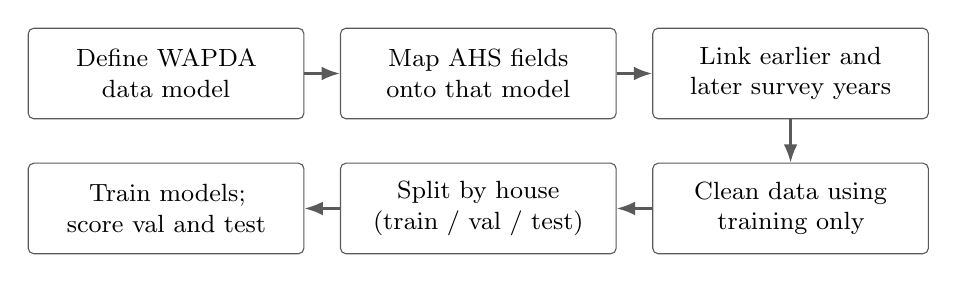
\begin{tikzpicture}[
  font=\small,
  box/.style={draw=rulegray, rounded corners=2pt, align=center, inner sep=5pt, text width=3.15cm, minimum height=1.15cm},
  arr/.style={-{Latex}, thick, rulegray}
]
\node[box] (s) {Define WAPDA\\data model};
\node[box, right=0.45cm of s] (a) {Map AHS fields\\onto that model};
\node[box, right=0.45cm of a] (h) {Link earlier and\\later survey years};
\node[box, below=0.55cm of h] (p) {Clean data using\\training only};
\node[box, below=0.55cm of a] (t) {Split by house\\(train / val / test)};
\node[box, below=0.55cm of s] (m) {Train models;\\score val and test};
\draw[arr] (s) -- (a);
\draw[arr] (a) -- (h);
\draw[arr] (h) -- (p);
\draw[arr] (p) -- (t);
\draw[arr] (t) -- (m);
\end{tikzpicture}
\caption{Project steps. First we fix the WAPDA data model. Then we map public survey data onto it.}
\label{fig:flow}
\end{figure}

\subsection{Models and how we choose a winner}

We compare three simple baselines and four learning models:

\begin{itemize}
  \item \textbf{Training median:} predict the middle cost from training.
  \item \textbf{Type median:} predict the middle cost for that building type.
  \item \textbf{Prior cost:} predict last survey's maintenance cost.
  \item \textbf{Learning models:} linear regression, random forest, gradient boosting [5]--[7], and XGBoost [8].
\end{itemize}

First we used fixed settings. Later we tuned tree settings on the validation set only (144 XGBoost trials; best: 200 trees, depth 4, learning rate 0.03). We also tried absolute-error training. We never tuned on the test set.

\textbf{Metrics in plain words:}
\begin{itemize}
  \item \textbf{MAE} = average dollar miss (main score). Lower is better.
  \item \textbf{RMSE} = similar, but big misses hurt more.
  \item \textbf{High-cost F1} = how well we find houses above USD~1{,}428. Higher is better.
\end{itemize}

Our written rule: pick by validation MAE. Also report the no-2023 test and high-cost F1. A learning model is ``promoted'' only if it wins validation MAE and is at least as good on the no-2023 test. A good test MAE alone is not enough.

\section{Implementation and results}

The code is a Python package named \texttt{caip\_maintenance}. Config files sit under \texttt{configs/}. Tests check that houses do not leak across splits and that cleaning uses training data only. The tables below use the saved experiment scores. We do not print private or row-level survey data here.

\subsection{Main comparison}

Table~\ref{tab:metrics} and Figures~\ref{fig:mae}--\ref{fig:tradeoff} show the key systems. ``Original'' = first feature set. ``Tuned'' = engineered features + validation search.

\begin{table}[ht]
\centering
\caption{Main scores in USD (except F1). Lower MAE/RMSE is better. Higher F1 is better. Median baselines have no F1 because they never flag high-cost houses.}
\label{tab:metrics}
\resizebox{\textwidth}{!}{%
\begin{tabular}{@{}lrrrrr@{}}
\toprule
System & Val.\ MAE & Test MAE & No-2023 MAE & Test RMSE & Test F1 \\
\midrule
Training median & 832.16 & 965.85 & 828.69 & 2360.09 & --- \\
Type median & \textbf{827.95} & 962.81 & \textbf{824.82} & 2361.65 & --- \\
Prior cost & 952.44 & 1058.25 & 936.53 & 2358.81 & \textbf{0.410} \\
Linear regression (orig.) & 849.50 & 950.91 & 833.34 & 2182.90 & 0.384 \\
Random forest (orig.) & 850.27 & 956.54 & 837.78 & 2188.13 & 0.397 \\
Gradient boosting (orig.) & 843.34 & 949.15 & 829.68 & 2188.68 & 0.356 \\
XGBoost (orig.) & 845.90 & 949.38 & 830.26 & 2189.87 & 0.386 \\
Random forest (tuned) & 841.23 & 946.57 & 828.18 & 2186.38 & 0.385 \\
Gradient boosting (tuned) & 841.16 & 945.27 & 826.76 & 2183.34 & 0.373 \\
XGBoost (tuned) & 838.83 & \textbf{944.34} & 825.35 & \textbf{2182.07} & 0.391 \\
XGBoost (absolute loss) & 778.41 & 899.07 & 767.77 & 2268.28 & 0.113 \\
\bottomrule
\end{tabular}}
\end{table}

\begin{figure}[ht]
\centering
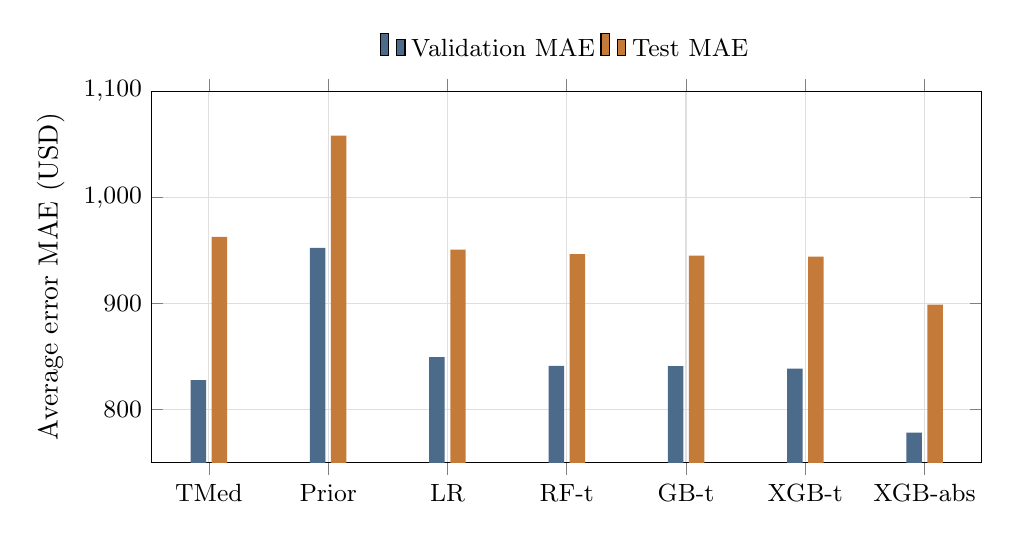
\begin{tikzpicture}
\begin{axis}[
  ybar,
  bar width=5.6pt,
  width=\textwidth,
  height=6.3cm,
  ylabel={Average error MAE (USD)},
  ymin=750, ymax=1100,
  symbolic x coords={TMed, Prior, LR, RF-t, GB-t, XGB-t, XGB-abs},
  xtick=data,
  xticklabel style={font=\small},
  legend style={at={(0.5,1.05)}, anchor=south, legend columns=2, draw=none, font=\small},
  grid=major,
  major grid style={gray!25},
  enlarge x limits=0.08,
  tick label style={font=\small},
]
\addplot[fill=barval, draw=none] coordinates {
  (TMed,827.95) (Prior,952.44) (LR,849.50) (RF-t,841.23) (GB-t,841.16) (XGB-t,838.83) (XGB-abs,778.41)
};
\addplot[fill=bartest, draw=none] coordinates {
  (TMed,962.81) (Prior,1058.25) (LR,950.91) (RF-t,946.57) (GB-t,945.27) (XGB-t,944.34) (XGB-abs,899.07)
};
\legend{Validation MAE, Test MAE}
\end{axis}
\end{tikzpicture}
\caption{Average error (MAE). Type median (TMed) is best on validation. Tuned XGBoost (XGB-t) is best on the test set among normal models. Absolute-error XGBoost (XGB-abs) has the lowest MAE but fails later on high-cost finding.}
\label{fig:mae}
\end{figure}

On validation, \textbf{type median} wins (827.95~USD). Tuned XGBoost is close (838.83~USD) but still about 11 dollars worse.

On the test set, \textbf{tuned XGBoost} wins among normal models (944.34~USD MAE, 2182.07~USD RMSE). That is about 18 dollars better than type median. Random forest and gradient boosting are close behind. Adding extra features did not help linear regression.

All methods look better when we remove 2023 rows. That mostly reflects the 2023 survey change, not a big model skill gap. Type median is still slightly best on that no-2023 test. So our written rule does \textbf{not} promote XGBoost as the official winner, even though it wins the full test set.

Learning models also cut RMSE a lot (about 2{,}360 down to about 2{,}182). That means they handle some very expensive cases better than a simple median, even when average error only improves a little.

\subsection{Finding expensive houses}

Median baselines never predict above USD~1{,}428, so they never mark a house as high cost.

Among scoring methods, \textbf{prior cost} is best at finding expensive houses (F1 = 0.410). Tuned XGBoost is close (F1 = 0.391). Absolute-error XGBoost looks good on MAE but is bad at this job (F1 = 0.113). It rarely predicts high values, so it misses most expensive houses (Table~\ref{tab:hc}, Figures~\ref{fig:f1}--\ref{fig:tradeoff}).

\begin{figure}[ht]
\centering
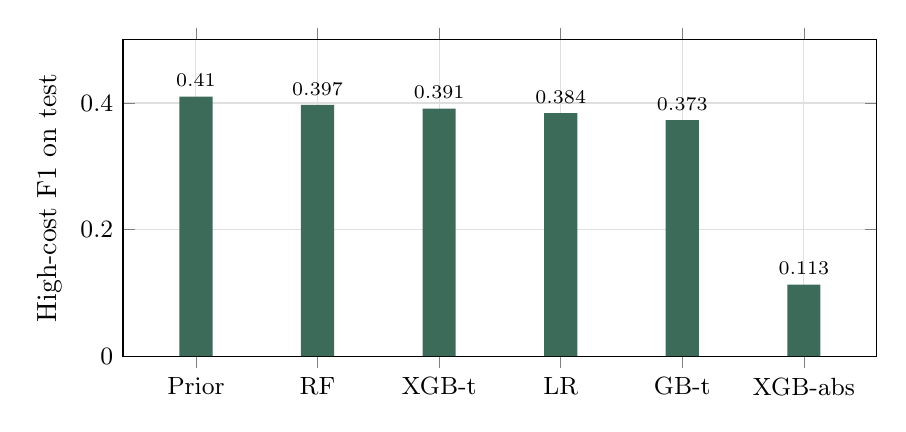
\begin{tikzpicture}
\begin{axis}[
  ybar,
  bar width=12pt,
  width=0.92\textwidth,
  height=5.6cm,
  ylabel={High-cost F1 on test},
  ymin=0, ymax=0.50,
  symbolic x coords={Prior, RF, XGB-t, LR, GB-t, XGB-abs},
  xtick=data,
  nodes near coords,
  nodes near coords style={font=\scriptsize, /pgf/number format/fixed, /pgf/number format/precision=3},
  enlarge x limits=0.12,
  grid=major,
  major grid style={gray!25},
  tick label style={font=\small},
]
\addplot[fill=barf1, draw=none] coordinates {
  (Prior,0.410) (RF,0.397) (XGB-t,0.391) (LR,0.384) (GB-t,0.373) (XGB-abs,0.113)
};
\end{axis}
\end{tikzpicture}
\caption{How well each method finds expensive houses. Prior cost is best. Absolute-error XGBoost is much worse.}
\label{fig:f1}
\end{figure}

\begin{table}[ht]
\centering
\caption{Finding houses above USD~1{,}428 on the test set.}
\label{tab:hc}
\begin{tabular}{@{}lrrr@{}}
\toprule
System & Precision & Recall & F1 \\
\midrule
Prior cost & 0.456 & 0.373 & 0.410 \\
Random forest (orig.) & 0.476 & 0.340 & 0.397 \\
XGBoost (tuned) & 0.502 & 0.320 & 0.391 \\
Linear regression (orig.) & 0.508 & 0.309 & 0.384 \\
Gradient boosting (tuned) & 0.515 & 0.293 & 0.373 \\
XGBoost (absolute loss) & 0.634 & 0.062 & 0.113 \\
\bottomrule
\end{tabular}
\end{table}

\begin{figure}[ht]
\centering
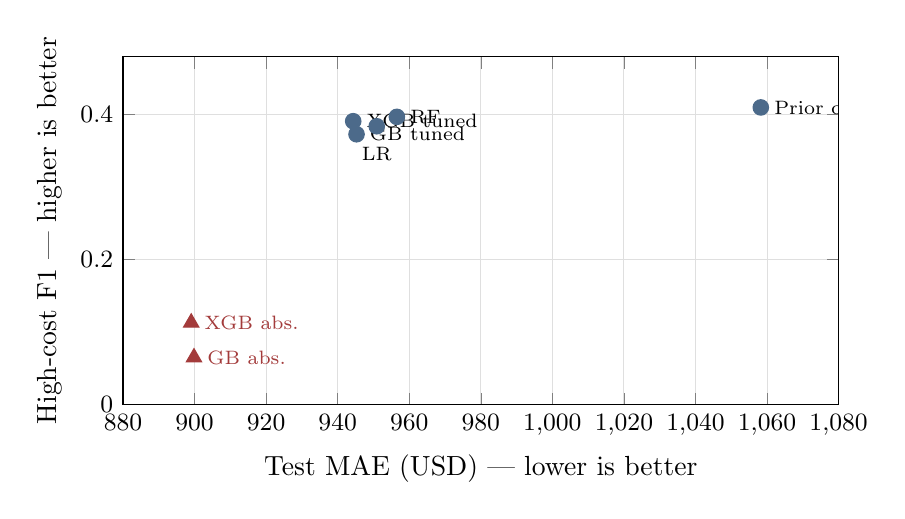
\begin{tikzpicture}
\begin{axis}[
  width=0.88\textwidth,
  height=6.0cm,
  xlabel={Test MAE (USD) --- lower is better},
  ylabel={High-cost F1 --- higher is better},
  xmin=880, xmax=1080,
  ymin=0, ymax=0.48,
  grid=major,
  major grid style={gray!25},
  tick label style={font=\small},
]
\addplot[only marks, mark=*, mark size=2.8pt, color=barval] coordinates {
  (1058.25, 0.410)
  (956.54, 0.397)
  (944.34, 0.391)
  (950.91, 0.384)
  (945.27, 0.373)
};
\node[font=\scriptsize, anchor=west] at (axis cs:1058.25,0.410) {\,Prior cost};
\node[font=\scriptsize, anchor=west] at (axis cs:956.54,0.397) {\,RF};
\node[font=\scriptsize, anchor=west] at (axis cs:944.34,0.391) {\,XGB tuned};
\node[font=\scriptsize, anchor=north] at (axis cs:950.91,0.368) {LR};
\node[font=\scriptsize, anchor=west] at (axis cs:945.27,0.373) {\,GB tuned};
\addplot[only marks, mark=triangle*, mark size=3.2pt, color=warnred] coordinates {
  (899.07, 0.113)
  (899.84, 0.065)
};
\node[font=\scriptsize, color=warnred, anchor=west] at (axis cs:899.07,0.113) {\,XGB abs.};
\node[font=\scriptsize, color=warnred, anchor=west] at (axis cs:899.84,0.065) {\,GB abs.};
\end{axis}
\end{tikzpicture}
\caption{Average error vs finding expensive houses. Absolute-error models move left (better MAE) but down (worse F1).}
\label{fig:tradeoff}
\end{figure}

Two quick checks: training on $\log(1+\mathrm{cost})$ helped middle errors but hurt high-cost finding, so we did not keep it. Removing past-cost features made gradient boosting worse (test MAE from 947.79 to 979.67). Past maintenance cost matters.

\subsection{What should we report?}

By our written rule:
\begin{itemize}
  \item \textbf{Best simple cost estimate:} type median.
  \item \textbf{Best simple high-cost signal:} prior cost.
\end{itemize}

If we only ask which learning model is strongest on the full test set \emph{and} still finds expensive houses, the answer is \textbf{tuned XGBoost}. That is a useful finding, not a claim that WAPDA should deploy it tomorrow.

\section{Discussion and conclusion}

A simple type median is hard to beat when the split is fair. House type already carries a lot of information. Learning models improve the test score a little and give a usable high-cost score. Absolute error reduces average miss but mostly stops warning about expensive houses. That is the wrong trade for prioritisation.

We need two different answers for two different jobs:
\begin{enumerate}
  \item \textbf{Budget number:} type median is strongest under the validation rule.
  \item \textbf{Which houses look expensive:} prior cost is the clearest simple signal; tuned XGBoost is the best learning compromise.
\end{enumerate}

The 2023 survey change shows why a second test without 2023 was needed. If recording rules change, every error number can move even when houses stay the same.

Privacy also shaped the work. Names, CNIC, phone numbers, salaries, and free-text remarks from WASC files are not in the training tables or this report. IDs are tokenized. Raw rows and trained model files are not in the email annex.

For real WAPDA use later, the useful part is the data model and the safe workflow, not these USD scores. WAPDA would still need linked work orders, verified costs, and clear coverage so ``zero cost'' is not confused with ``missing data.''

The web app is future work.

\textbf{Final takeaway.} The dataset is made on the WAPDA data model and filled with mapped AHS records because WAPDA work-order files were not available. Type median is the main cost baseline. Prior cost is the main high-cost baseline. Tuned XGBoost is the best learning model on the full test set that still finds expensive houses. Absolute-error models lower MAE but miss most expensive houses. None of these is a validated WAPDA operational forecast.

\section*{References}
\begin{enumerate}[leftmargin=1.6em,itemsep=0.25em,label={[\arabic*]}]
  \item U.S. Census Bureau and U.S. Department of Housing and Urban Development, ``American Housing Survey: 2023 Data,'' 2023. [Online]. Available: \url{https://www.census.gov/programs-surveys/ahs/data/2023.html}
  \item U.S. Census Bureau, ``American Housing Survey Codebooks.'' [Online]. Available: \url{https://www.census.gov/programs-surveys/ahs/tech-documentation/codebooks.html}
  \item U.S. Census Bureau, \textit{Sample Case History File 2015 to 2023}. [Online]. Available: \path{https://www2.census.gov/programs-surveys/ahs/documentation/}
  \item U.S. Census Bureau, \textit{2023 AHS Historical Changes}, 2023. [Online]. Available: \url{https://www2.census.gov/programs-surveys/ahs/2023/2023\%20AHS\%20Historical\%20Changes.pdf}
  \item L. Breiman, ``Random forests,'' \textit{Machine Learning}, vol.~45, no.~1, pp.~5--32, 2001.
  \item J.~H. Friedman, ``Greedy function approximation: A gradient boosting machine,'' \textit{The Annals of Statistics}, vol.~29, no.~5, pp.~1189--1232, 2001.
  \item F. Pedregosa \textit{et al.}, ``Scikit-learn: Machine learning in Python,'' \textit{Journal of Machine Learning Research}, vol.~12, pp.~2825--2830, 2011.
  \item T. Chen and C. Guestrin, ``XGBoost: A scalable tree boosting system,'' in \textit{Proc.\ 22nd ACM SIGKDD}, 2016, pp.~785--794.
\end{enumerate}

\appendix
\section{Code annex (summary)}
Full code is in \texttt{caip\_code\_annex.zip}. The separate test file is \texttt{caip\_final\_source.py}. Neither file has raw WASC or AHS row data.

Example checks from the project root:

{\small
\begin{verbatim}
PYTHONPATH=src .venv/bin/python -m caip_maintenance.data \
  audit-experiment --experiment ahs-baselines-models-v1
PYTHONPATH=src .venv/bin/python -m caip_maintenance.data \
  audit-ahs-xgboost-tuning --experiment ahs-xgboost-tuning-v1
.venv/bin/python -m unittest discover -s tests -v
\end{verbatim}
}

\end{document}
